\documentclass[12pt,]{article}
\usepackage{lmodern}
\usepackage{amssymb,amsmath}
\usepackage{ifxetex,ifluatex}
\usepackage{fixltx2e} % provides \textsubscript
\ifnum 0\ifxetex 1\fi\ifluatex 1\fi=0 % if pdftex
  \usepackage[T1]{fontenc}
  \usepackage[utf8]{inputenc}
\else % if luatex or xelatex
  \ifxetex
    \usepackage{mathspec}
  \else
    \usepackage{fontspec}
  \fi
  \defaultfontfeatures{Ligatures=TeX,Scale=MatchLowercase}
\fi
% use upquote if available, for straight quotes in verbatim environments
\IfFileExists{upquote.sty}{\usepackage{upquote}}{}
% use microtype if available
\IfFileExists{microtype.sty}{%
\usepackage{microtype}
\UseMicrotypeSet[protrusion]{basicmath} % disable protrusion for tt fonts
}{}
\usepackage[margin=1in]{geometry}
\usepackage{hyperref}
\PassOptionsToPackage{usenames,dvipsnames}{color} % color is loaded by hyperref
\hypersetup{unicode=true,
            pdftitle={Data, Research, and Visualization Unit},
            colorlinks=true,
            linkcolor=Maroon,
            citecolor=Blue,
            urlcolor=blue,
            breaklinks=true}
\urlstyle{same}  % don't use monospace font for urls
\usepackage{color}
\usepackage{fancyvrb}
\newcommand{\VerbBar}{|}
\newcommand{\VERB}{\Verb[commandchars=\\\{\}]}
\DefineVerbatimEnvironment{Highlighting}{Verbatim}{commandchars=\\\{\}}
% Add ',fontsize=\small' for more characters per line
\usepackage{framed}
\definecolor{shadecolor}{RGB}{248,248,248}
\newenvironment{Shaded}{\begin{snugshade}}{\end{snugshade}}
\newcommand{\AlertTok}[1]{\textcolor[rgb]{0.94,0.16,0.16}{#1}}
\newcommand{\AnnotationTok}[1]{\textcolor[rgb]{0.56,0.35,0.01}{\textbf{\textit{#1}}}}
\newcommand{\AttributeTok}[1]{\textcolor[rgb]{0.77,0.63,0.00}{#1}}
\newcommand{\BaseNTok}[1]{\textcolor[rgb]{0.00,0.00,0.81}{#1}}
\newcommand{\BuiltInTok}[1]{#1}
\newcommand{\CharTok}[1]{\textcolor[rgb]{0.31,0.60,0.02}{#1}}
\newcommand{\CommentTok}[1]{\textcolor[rgb]{0.56,0.35,0.01}{\textit{#1}}}
\newcommand{\CommentVarTok}[1]{\textcolor[rgb]{0.56,0.35,0.01}{\textbf{\textit{#1}}}}
\newcommand{\ConstantTok}[1]{\textcolor[rgb]{0.00,0.00,0.00}{#1}}
\newcommand{\ControlFlowTok}[1]{\textcolor[rgb]{0.13,0.29,0.53}{\textbf{#1}}}
\newcommand{\DataTypeTok}[1]{\textcolor[rgb]{0.13,0.29,0.53}{#1}}
\newcommand{\DecValTok}[1]{\textcolor[rgb]{0.00,0.00,0.81}{#1}}
\newcommand{\DocumentationTok}[1]{\textcolor[rgb]{0.56,0.35,0.01}{\textbf{\textit{#1}}}}
\newcommand{\ErrorTok}[1]{\textcolor[rgb]{0.64,0.00,0.00}{\textbf{#1}}}
\newcommand{\ExtensionTok}[1]{#1}
\newcommand{\FloatTok}[1]{\textcolor[rgb]{0.00,0.00,0.81}{#1}}
\newcommand{\FunctionTok}[1]{\textcolor[rgb]{0.00,0.00,0.00}{#1}}
\newcommand{\ImportTok}[1]{#1}
\newcommand{\InformationTok}[1]{\textcolor[rgb]{0.56,0.35,0.01}{\textbf{\textit{#1}}}}
\newcommand{\KeywordTok}[1]{\textcolor[rgb]{0.13,0.29,0.53}{\textbf{#1}}}
\newcommand{\NormalTok}[1]{#1}
\newcommand{\OperatorTok}[1]{\textcolor[rgb]{0.81,0.36,0.00}{\textbf{#1}}}
\newcommand{\OtherTok}[1]{\textcolor[rgb]{0.56,0.35,0.01}{#1}}
\newcommand{\PreprocessorTok}[1]{\textcolor[rgb]{0.56,0.35,0.01}{\textit{#1}}}
\newcommand{\RegionMarkerTok}[1]{#1}
\newcommand{\SpecialCharTok}[1]{\textcolor[rgb]{0.00,0.00,0.00}{#1}}
\newcommand{\SpecialStringTok}[1]{\textcolor[rgb]{0.31,0.60,0.02}{#1}}
\newcommand{\StringTok}[1]{\textcolor[rgb]{0.31,0.60,0.02}{#1}}
\newcommand{\VariableTok}[1]{\textcolor[rgb]{0.00,0.00,0.00}{#1}}
\newcommand{\VerbatimStringTok}[1]{\textcolor[rgb]{0.31,0.60,0.02}{#1}}
\newcommand{\WarningTok}[1]{\textcolor[rgb]{0.56,0.35,0.01}{\textbf{\textit{#1}}}}
\usepackage{graphicx,grffile}
\makeatletter
\def\maxwidth{\ifdim\Gin@nat@width>\linewidth\linewidth\else\Gin@nat@width\fi}
\def\maxheight{\ifdim\Gin@nat@height>\textheight\textheight\else\Gin@nat@height\fi}
\makeatother
% Scale images if necessary, so that they will not overflow the page
% margins by default, and it is still possible to overwrite the defaults
% using explicit options in \includegraphics[width, height, ...]{}
\setkeys{Gin}{width=\maxwidth,height=\maxheight,keepaspectratio}
\IfFileExists{parskip.sty}{%
\usepackage{parskip}
}{% else
\setlength{\parindent}{0pt}
\setlength{\parskip}{6pt plus 2pt minus 1pt}
}
\setlength{\emergencystretch}{3em}  % prevent overfull lines
\providecommand{\tightlist}{%
  \setlength{\itemsep}{0pt}\setlength{\parskip}{0pt}}
\setcounter{secnumdepth}{0}
% Redefines (sub)paragraphs to behave more like sections
\ifx\paragraph\undefined\else
\let\oldparagraph\paragraph
\renewcommand{\paragraph}[1]{\oldparagraph{#1}\mbox{}}
\fi
\ifx\subparagraph\undefined\else
\let\oldsubparagraph\subparagraph
\renewcommand{\subparagraph}[1]{\oldsubparagraph{#1}\mbox{}}
\fi

%%% Use protect on footnotes to avoid problems with footnotes in titles
\let\rmarkdownfootnote\footnote%
\def\footnote{\protect\rmarkdownfootnote}

%%% Change title format to be more compact
\usepackage{titling}

% Create subtitle command for use in maketitle
\newcommand{\subtitle}[1]{
  \posttitle{
    \begin{center}\large#1\end{center}
    }
}

\setlength{\droptitle}{-2em}

  \title{Data, Research, and Visualization Unit}
    \pretitle{\vspace{\droptitle}\centering\huge}
  \posttitle{\par}
    \author{}
    \preauthor{}\postauthor{}
    \date{}
    \predate{}\postdate{}
  
\usepackage{booktabs}
\usepackage{longtable}
\usepackage{array}
\usepackage{multirow}
\usepackage[table]{xcolor}
\usepackage{wrapfig}
\usepackage{float}
\usepackage{colortbl}
\usepackage{pdflscape}
\usepackage{tabu}
\usepackage{threeparttable}
\usepackage{threeparttablex}
\usepackage[normalem]{ulem}
\usepackage{makecell}

\usepackage{pdflscape}
\newcommand{\blandscape}{\begin{landscape}}
\newcommand{\elandscape}{\end{landscape}}

\begin{document}
\maketitle

\hypertarget{executive-summary}{%
\section{Executive Summary}\label{executive-summary}}

The department should invest staffing resources into a Data, Research,
and Visualization unit that, in addition to compiling AOIC statistics,
works with the
\href{https://www.cookcountyil.gov/agency/geographic-information-systems-gis-0}{Cook
County Geographic Information Systems Department} to create new, data
driven tools and supplement the dashboards of created by
\href{https://www.cfive.com/products/supervisor/}{CFive's Supervisor}.
This unit, staffed by sworn staff and support professionals would use
Excel, \href{https://www.r-project.org}{R}, and
\href{https://www.esri.com/en-us/what-is-gis/overview}{GIS} to collect,
clean, and analyze data to ensure the department is maximizing the
investment in \emph{CFive Supervisor.}

\hypertarget{the-issue}{%
\section{The Issue}\label{the-issue}}

To demonstrate the need of a new Data, Research, and Visualization unit,
consider the current report for AOIC. Currently, the AOIC Stats are
presented in the following format:

\rowcolors{2}{gray!6}{white}
\begin{table}[!h]

\caption{\label{tab:first_8}First Eight Columns of CFive Supervisor}
\centering
\resizebox{\linewidth}{!}{
\begin{tabular}[t]{l|l|l|l|l|l|l|l}
\hiderowcolors
\hline
X\_\_1 & X\_\_2 & X\_\_3 & X\_\_4 & X\_\_5 & X\_\_6 & X\_\_7 & X\_\_8\\
\hline
\showrowcolors
Terri Griffin & NA & NA & NA & NA & NA & NA & NA\\
\hline
Police District 17, 14, 18-20 - Cal. 58, 60 & NA & NA & NA & NA & NA & NA & NA\\
\hline
Diane Bufano & NA & NA & NA & NA & NA & NA & NA\\
\hline
NA & Laura Donnelly & Andrea Korte & Michelle Malave & Amy O'Rourke & Yvonne Pulido & Diane Bufano & NA\\
\hline
Total Caseload & 17 & 9 & 20 & 13 & 21 & 1 & NA\\
\hline
YASI HIGH & 4 & 2 & 3 & 2 & 5 & NA & NA\\
\hline
\end{tabular}}
\end{table}
\rowcolors{2}{white}{white}

Of course, the Excel report is more aesthetically pleasing, but the
overall format is identical: Multiple units on the document, multiple
breakdowns of stats collected, and multiple types of observations.

The first eight columns are the POs, per unit, at a glance, depending on
the number of POs in the unit and the number of cases assigned to the
Supervisor.

\rowcolors{2}{gray!6}{white}
\begin{table}[H]

\caption{\label{tab:9_11}Caseload Aggregate Data}
\centering
\begin{tabular}[t]{l|l|l}
\hiderowcolors
\hline
X\_\_9 & X\_\_10 & X\_\_11\\
\hline
\showrowcolors
NA & NA & NA\\
\hline
NA & NA & NA\\
\hline
NA & NA & NA\\
\hline
CASELOAD TOTAL & AVERAGE CASELOAD & Total P.Os\\
\hline
81 & 16 & 5\\
\hline
16 & NA & NA\\
\hline
\end{tabular}
\end{table}
\rowcolors{2}{white}{white}

Columns 9 through 10 are aggregates of the previous unit data.

\rowcolors{2}{gray!6}{white}
\begin{table}[H]

\caption{\label{tab:12-19}VOPs and Caseload Averages}
\centering
\resizebox{\linewidth}{!}{
\begin{tabular}[t]{l|l|r|r|l|r|l|r}
\hiderowcolors
\hline
X\_\_12 & X\_\_13 & VOP'S FILED BY UNIT & Baseline(Average for the month) & Caseload size & Dept average caseload size & Average Caseload Size for Unit & Average Caseload Size\\
\hline
\showrowcolors
1 & SPO Bufano & 2 & 2 & 81 & 72 & 16 & 16\\
\hline
2 & SPO Carter & 2 & 2 & 29 & 72 & 14.5 & 16\\
\hline
3 & SPO Flanagan & 2 & 2 & 59 & 72 & 14 & 16\\
\hline
4 & SPO Alejo & 3 & 2 & 58 & 72 & 11.6 & 16\\
\hline
5 & SPO Herner & 1 & 2 & 46 & 72 & 15.333333333333334 & 16\\
\hline
6 & SPO Moore & 4 & 2 & 55 & 72 & 11 & 16\\
\hline
\end{tabular}}
\end{table}
\rowcolors{2}{white}{white}

The remaining seven columns are a mishmash of stats by unit and
department.

Presenting AOIC data in this fashion limits further investigation of
data. Multiple spreadsheets must be created to combine data for
month-month comparisons, and compiling said spreadsheets increases the
chances of errors due to spelling mistakes, accidentally deleting
spreadsheet structure, or over-writing spreadsheets while saving them.

Fortunately, \href{https://www.cfive.com/products/supervisor/}{CFive's
Supervisor} will be able to solve most of these data collection issues.
As of the current understanding of the Statement of Work,
\emph{Supervisor} will pull these necessary numbers from the system as a
standard report. Another possible scenario is SPOs will complete a
\emph{Supervisor} based form that will guide the creation of the report.
Regardless, the method in which the AOIC Stats are gathered and
presented will change. Unfortunately, the reporting features are not
completed and not available for preview.

This gap presents an opportunity for the department to reformat any and
all of the statistical forms and reports, starting with the AOIC
reports, to ensure our data and visualization needs are not just met,
but exceeded. The \emph{Supervisor's Go-Live }\footnote{As of this
  writing, Go-Live is set for March 29, 2019} date provides an incentive
to get this material completed quickly.

\hypertarget{new-format-and-methods-the-solution}{%
\section{New Format and Methods: The
Solution}\label{new-format-and-methods-the-solution}}

Implementing \href{http://vita.had.co.nz/papers/tidy-data.html}{tidy
data} is the first step to any transformation to a data-driven office.
Tidy data is short hand for:

\begin{itemize}
\tightlist
\item
  Columns are single variable
\item
  Rows are single observation
\item
  Each observational unit forms a table
\end{itemize}

Currently, the AOIC spreadsheets violates all of the rules of tidy data.
The easiest example to understand is how each sheet is a collection of
observations and aggregates across units. In truth, each geographic unit
should have their own worksheet, with separate worksheets for averages
and other calculated variables. It appears that the sheets follow the
first and second rules; however, considering what is being tracked, the
columns and rows are transposed. Put differently, in the current format,
POs are variables when they they are actually tracking observations. In
tidy terms this makes them \emph{rows.}

\hypertarget{gbo-as-a-demo}{%
\subsection{GBO As a Demo}\label{gbo-as-a-demo}}

For example, take the GBO unit. On the standard AOIC spreadsheet, GBO's
stats are between rows 401 and 418:

\rowcolors{2}{lightgray}{white}
\begin{table}[!h]

\caption{\label{tab:gbo_demo}September, 2018}
\centering
\resizebox{\linewidth}{!}{
\begin{tabular}[t]{llllllll}
\hiderowcolors
\toprule
AOIC\_Stat & PO\_Stat1 & PO\_Stat2 & PO\_Stat3 & PO\_Stat4 & PO\_Stat5 & PO\_Stat6 & PO\_Stat7\\
\midrule
\showrowcolors
Melissa Spooner & NA & NA & NA & NA & NA & NA & NA\\
Police district 2 - Cal 55 & NA & NA & NA & NA & NA & NA & NA\\
Lloyd Marshall & NA & NA & NA & NA & NA & NA & NA\\
NA & Ernest Jones & Michael Muhammad & Rodney Purdy-Blake & James Smith & ADMIN & NA & NA\\
Total Caseload & 16 & 17 & 15 & 16 & NA & NA & NA\\
\addlinespace
YASI HIGH & 7 & 8 & 4 & 1 & NA & NA & NA\\
YASI MOD & 6 & 6 & 7 & 9 & NA & NA & NA\\
YASI LOW & 1 & 2 & 2 & 3 & NA & NA & NA\\
YASI UNCLASSIFIED & 2 & 1 & 2 & 3 & NA & NA & NA\\
Scheduled Termination & 2 & 1 & 1 & 1 & NA & NA & NA\\
\addlinespace
Early Termination & NA & NA & NA & NA & NA & NA & NA\\
Revoked-Technical/DOC-IDJJ & NA & NA & NA & NA & NA & NA & NA\\
Revoked-new offense/DOC-IDJJ & NA & NA & NA & NA & NA & NA & NA\\
Unsatisfactory termination & NA & NA & NA & NA & NA & NA & NA\\
Transferred out & NA & NA & NA & NA & NA & NA & NA\\
\addlinespace
Social investigation & NA & NA & NA & NA & NA & NA & NA\\
Supplemental social & NA & NA & NA & NA & NA & NA & NA\\
VOP Filed & NA & NA & NA & NA & NA & NA & NA\\
\bottomrule
\end{tabular}}
\end{table}
\rowcolors{2}{white}{white}

At a glance, one can see how individual officers case loads have changed
over the previous month. However, if one was to compare GBO and
Lawndale(rows 201-218), the issue with messy data becomes apparent:

\hypertarget{gbo-and-lawndale}{%
\subsection{GBO and Lawndale}\label{gbo-and-lawndale}}

\rowcolors{2}{lightgray}{white}
\begin{table}[!h]

\caption{\label{tab:GBO_and_Lawndale}GBO and Lawndale: September, 2018}
\centering
\resizebox{\linewidth}{!}{
\begin{tabular}[t]{llllllll}
\hiderowcolors
\toprule
AOIC\_Stat & PO\_Stat1 & PO\_Stat2 & PO\_Stat3 & PO\_Stat4 & PO\_Stat5 & PO\_Stat6 & PO\_Stat7\\
\midrule
\showrowcolors
Melissa Spooner & NA & NA & NA & NA & NA & NA & NA\\
Police district 2 - Cal 55 & NA & NA & NA & NA & NA & NA & NA\\
Lloyd Marshall & NA & NA & NA & NA & NA & NA & NA\\
NA & Ernest Jones & Michael Muhammad & Rodney Purdy-Blake & James Smith & ADMIN & NA & NA\\
Total Caseload & 16 & 17 & 15 & 16 & NA & NA & NA\\
\addlinespace
YASI HIGH & 7 & 8 & 4 & 1 & NA & NA & NA\\
YASI MOD & 6 & 6 & 7 & 9 & NA & NA & NA\\
YASI LOW & 1 & 2 & 2 & 3 & NA & NA & NA\\
YASI UNCLASSIFIED & 2 & 1 & 2 & 3 & NA & NA & NA\\
Scheduled Termination & 2 & 1 & 1 & 1 & NA & NA & NA\\
\addlinespace
Early Termination & NA & NA & NA & NA & NA & NA & NA\\
Revoked-Technical/DOC-IDJJ & NA & NA & NA & NA & NA & NA & NA\\
Revoked-new offense/DOC-IDJJ & NA & NA & NA & NA & NA & NA & NA\\
Unsatisfactory termination & NA & NA & NA & NA & NA & NA & NA\\
Transferred out & NA & NA & NA & NA & NA & NA & NA\\
\addlinespace
Social investigation & NA & NA & NA & NA & NA & NA & NA\\
Supplemental social & NA & NA & NA & NA & NA & NA & NA\\
VOP Filed & NA & NA & NA & NA & NA & NA & NA\\
Jose Isais & NA & NA & NA & NA & NA & NA & NA\\
Polce Distrct 11 - Cal. 57 & NA & NA & NA & NA & NA & NA & NA\\
\addlinespace
Aaron Campbell & NA & NA & NA & NA & NA & NA & NA\\
NA & Laterrian Hill & Rance Hopkins* & Pamela Hudson & Tesa Newton-Hart & Kenneth Ollins & Campbell & NA\\
Total Caseload & 27 & 31 & 23 & 22 & 26 & 1 & NA\\
YASI HIGH & 9 & NA & 6 & 10 & 3 & NA & NA\\
YASI MOD & 10 & NA & 9 & 5 & 11 & 1 & NA\\
\addlinespace
YASI LOW & 8 & NA & 3 & 6 & 9 & NA & NA\\
YASI UNCLASSIFIED & NA & 31 & 5 & 1 & 3 & NA & NA\\
Scheduled Termination & 2 & NA & 1 & 2 & NA & NA & NA\\
Early Termination & NA & NA & NA & NA & NA & NA & NA\\
Revoked-Technical/DOC-IDJJ & NA & NA & NA & NA & NA & NA & NA\\
\addlinespace
Revoked-new offense/DOC-IDJJ & NA & NA & NA & NA & NA & NA & NA\\
Unsatisfactory termination & 2 & NA & NA & NA & 1 & NA & NA\\
Transferred out & NA & 9 & NA & NA & NA & NA & NA\\
Social investigation & NA & 8 & NA & NA & NA & NA & NA\\
Supplemental social & NA & NA & NA & NA & NA & NA & NA\\
VOP Filed & 1 & NA & NA & NA & NA & 1 & NA\\
\bottomrule
\end{tabular}}
\end{table}
\rowcolors{2}{white}{white}

\newpage

With only one additional unit, it is relatively easy to compare and
contrast intra-unit data. It does require a reader to track data
vertically and horizontally. It is far from ideal. Specifically, one has
to read horizontally and vertically to compare baseline data month over
month. With each unit added to this format, the more difficult it
becomes to not just compare data points, but to find data points. For
example:

\rowcolors{2}{lightgray}{white}
\begin{table}[H]

\caption{\label{tab:GBO_Lawndale_and_53}GBO, Lawndale, and 8th District: September, 2018}
\centering
\resizebox{\linewidth}{!}{
\begin{tabular}[t]{llllllll}
\hiderowcolors
\toprule
AOIC\_Stat & PO\_Stat1 & PO\_Stat2 & PO\_Stat3 & PO\_Stat4 & PO\_Stat5 & PO\_Stat6 & PO\_Stat7\\
\midrule
\showrowcolors
Melissa Spooner & NA & NA & NA & NA & NA & NA & NA\\
Police district 2 - Cal 55 & NA & NA & NA & NA & NA & NA & NA\\
Lloyd Marshall & NA & NA & NA & NA & NA & NA & NA\\
NA & Ernest Jones & Michael Muhammad & Rodney Purdy-Blake & James Smith & ADMIN & NA & NA\\
Total Caseload & 16 & 17 & 15 & 16 & NA & NA & NA\\
\addlinespace
YASI HIGH & 7 & 8 & 4 & 1 & NA & NA & NA\\
YASI MOD & 6 & 6 & 7 & 9 & NA & NA & NA\\
YASI LOW & 1 & 2 & 2 & 3 & NA & NA & NA\\
YASI UNCLASSIFIED & 2 & 1 & 2 & 3 & NA & NA & NA\\
Scheduled Termination & 2 & 1 & 1 & 1 & NA & NA & NA\\
\addlinespace
Early Termination & NA & NA & NA & NA & NA & NA & NA\\
Revoked-Technical/DOC-IDJJ & NA & NA & NA & NA & NA & NA & NA\\
Revoked-new offense/DOC-IDJJ & NA & NA & NA & NA & NA & NA & NA\\
Unsatisfactory termination & NA & NA & NA & NA & NA & NA & NA\\
Transferred out & NA & NA & NA & NA & NA & NA & NA\\
\addlinespace
Social investigation & NA & NA & NA & NA & NA & NA & NA\\
Supplemental social & NA & NA & NA & NA & NA & NA & NA\\
VOP Filed & NA & NA & NA & NA & NA & NA & NA\\
Jose Isais & NA & NA & NA & NA & NA & NA & NA\\
Polce Distrct 11 - Cal. 57 & NA & NA & NA & NA & NA & NA & NA\\
\addlinespace
Aaron Campbell & NA & NA & NA & NA & NA & NA & NA\\
NA & Laterrian Hill & Rance Hopkins* & Pamela Hudson & Tesa Newton-Hart & Kenneth Ollins & Campbell & NA\\
Total Caseload & 27 & 31 & 23 & 22 & 26 & 1 & NA\\
YASI HIGH & 9 & NA & 6 & 10 & 3 & NA & NA\\
YASI MOD & 10 & NA & 9 & 5 & 11 & 1 & NA\\
\addlinespace
YASI LOW & 8 & NA & 3 & 6 & 9 & NA & NA\\
YASI UNCLASSIFIED & NA & 31 & 5 & 1 & 3 & NA & NA\\
Scheduled Termination & 2 & NA & 1 & 2 & NA & NA & NA\\
Early Termination & NA & NA & NA & NA & NA & NA & NA\\
Revoked-Technical/DOC-IDJJ & NA & NA & NA & NA & NA & NA & NA\\
\addlinespace
Revoked-new offense/DOC-IDJJ & NA & NA & NA & NA & NA & NA & NA\\
Unsatisfactory termination & 2 & NA & NA & NA & 1 & NA & NA\\
Transferred out & NA & 9 & NA & NA & NA & NA & NA\\
Social investigation & NA & 8 & NA & NA & NA & NA & NA\\
Supplemental social & NA & NA & NA & NA & NA & NA & NA\\
\addlinespace
VOP Filed & 1 & NA & NA & NA & NA & 1 & NA\\
Ore Jones, III & NA & NA & NA & NA & NA & NA & NA\\
PolicePolice District 10 - Cal. 53 & NA & NA & NA & NA & NA & NA & NA\\
Bennie Blair & NA & NA & NA & NA & NA & NA & NA\\
NA & Cedric Bell & Tyrone Hutson & Tandra Tyler & Robert Hillyer & Bennie Blair & NA & NA\\
\addlinespace
Total Caseload & 21 & 21 & 19 & 11 & 2 & NA & NA\\
YASI HIGH & NA & 5 & 2 & 4 & 2 & NA & NA\\
YASI MOD & 11 & 4 & 10 & 5 & NA & NA & NA\\
YASI LOW & 2 & 7 & 4 & 2 & NA & NA & NA\\
YASI UNCLASSIFIED & 8 & 5 & 3 & NA & NA & NA & NA\\
\addlinespace
Scheduled Termination & 1 & 2 & 1 & NA & NA & NA & NA\\
Early Termination & NA & NA & NA & NA & NA & NA & NA\\
Revoked-Technical/DOC-IDJJ & NA & NA & NA & NA & NA & NA & NA\\
Revoked-new offense/DOC-IDJJ & 1 & NA & NA & NA & NA & NA & NA\\
Unsatisfactory termination & 1 & NA & NA & NA & NA & NA & NA\\
\addlinespace
Transferred out & 1 & 1 & 3 & 1 & NA & NA & NA\\
Social investigation & NA & NA & 1 & NA & NA & NA & NA\\
Supplemental social & NA & 2 & 2 & 1 & NA & NA & NA\\
VOP Filed & NA & NA & NA & 1 & NA & NA & NA\\
\bottomrule
\end{tabular}}
\end{table}
\rowcolors{2}{white}{white}

The current excel format solves this issue by adding two or three empty
rows; however, the lack of standard difference between rows makes
machine based analysis slower and more time consuming. It also makes
plotting data exceptionally difficult.

\newpage

\begin{landscape}

\hypertarget{new-format}{%
\subsection{New format}\label{new-format}}

The solution looks like this:

\rowcolors{2}{lightgray}{white}
\begin{table}[!h]

\caption{\label{tab:tidy}GBO: September, 2018}
\centering
\resizebox{\linewidth}{!}{
\begin{tabular}[t]{lrrrrrrrrrrrrrlll}
\hiderowcolors
\toprule
PO\_Name & Early Termination & Revoked-new offense/DOC-IDJJ & Revoked-Technical/DOC-IDJJ & Scheduled Termination & Social investigation & Supplemental social & Transferred out & Unsatisfactory termination & VOP Filed & YASI HIGH & YASI LOW & YASI MOD & YASI UNCLASSIFIED & Unit & SPO & DCPO\\
\midrule
\showrowcolors
ADMIN & 0 & 0 & 0 & 0 & 0 & 0 & 0 & 0 & 0 & 0 & 0 & 0 & 0 & Police district 2 - Cal 55 & Lloyd Marshall & Melissa Spooner\\
Ernest Jones & 0 & 0 & 0 & 2 & 0 & 0 & 0 & 0 & 0 & 7 & 1 & 6 & 2 & Police district 2 - Cal 55 & Lloyd Marshall & Melissa Spooner\\
James Smith & 0 & 0 & 0 & 1 & 0 & 0 & 0 & 0 & 0 & 1 & 3 & 9 & 3 & Police district 2 - Cal 55 & Lloyd Marshall & Melissa Spooner\\
Michael Muhammad & 0 & 0 & 0 & 1 & 0 & 0 & 0 & 0 & 0 & 8 & 2 & 6 & 1 & Police district 2 - Cal 55 & Lloyd Marshall & Melissa Spooner\\
Rodney Purdy-Blake & 0 & 0 & 0 & 1 & 0 & 0 & 0 & 0 & 0 & 4 & 2 & 7 & 2 & Police district 2 - Cal 55 & Lloyd Marshall & Melissa Spooner\\
\bottomrule
\end{tabular}}
\end{table}
\rowcolors{2}{white}{white}

This create a difficult-to-read 17 columns\footnote{The columns are:
  \emph{PO\_Name, Early Termination, Revoked-new offense/DOC-IDJJ,
  Revoked-Technical/DOC-IDJJ, Scheduled Termination, Social
  investigation, Supplemental social, Transferred out, Unsatisfactory
  termination, VOP Filed, YASI HIGH, YASI LOW, YASI MOD, YASI
  UNCLASSIFIED, Unit, SPO, DCPO}} wide table which is difficult to read
on paper. The difficulty is mitigated because of the ability to to zoom
in on particular areas of interest, either by automating the reports to
fit particular needs or through web based technologies (which will be
discussed later.) It is also possible to filter data by specific
variables. For example, if one just wanted YASI data:

\rowcolors{2}{lightgray}{white}
\begin{table}[!h]

\caption{\label{tab:yasi}Case Totals, GBO: September, 2018}
\centering
\resizebox{\linewidth}{!}{
\begin{tabular}[t]{lrrrrr}
\hiderowcolors
\toprule
PO\_Name & High & Mod & Low & Unclassified & Total\\
\midrule
\showrowcolors
ADMIN & 0 & 0 & 0 & 0 & 0\\
Ernest Jones & 7 & 6 & 1 & 2 & 16\\
James Smith & 1 & 9 & 3 & 3 & 16\\
Michael Muhammad & 8 & 6 & 2 & 1 & 17\\
Rodney Purdy-Blake & 4 & 7 & 2 & 2 & 15\\
\bottomrule
\end{tabular}}
\end{table}
\rowcolors{2}{white}{white}

\newpage

Once the Excel data is in this format, it is easier to analyse. For
instance, take a table of two units arranged by High risk cases:

\rowcolors{2}{lightgray}{white}
\begin{table}[!h]

\caption{\label{tab:tidy_2}GBO and Lawndale by High Risk: September, 2018}
\centering
\resizebox{\linewidth}{!}{
\begin{tabular}[t]{lrrrrrrrrrrrrrlll}
\hiderowcolors
\toprule
PO\_Name & Early Termination & Revoked-new offense/DOC-IDJJ & Revoked-Technical/DOC-IDJJ & Scheduled Termination & Social investigation & Supplemental social & Transferred out & Unsatisfactory termination & VOP Filed & YASI HIGH & YASI LOW & YASI MOD & YASI UNCLASSIFIED & Unit & SPO & DCPO\\
\midrule
\showrowcolors
Tesa Newton-Hart & 0 & 0 & 0 & 2 & 0 & 0 & 0 & 0 & 0 & 10 & 6 & 5 & 1 & Polce Distrct 11 - Cal. 57 & Aaron Campbell & Jose Isais\\
Laterrian Hill & 0 & 0 & 0 & 2 & 0 & 0 & 0 & 2 & 1 & 9 & 8 & 10 & 0 & Polce Distrct 11 - Cal. 57 & Aaron Campbell & Jose Isais\\
Michael Muhammad & 0 & 0 & 0 & 1 & 0 & 0 & 0 & 0 & 0 & 8 & 2 & 6 & 1 & Police district 2 - Cal 55 & Lloyd Marshall & Melissa Spooner\\
Ernest Jones & 0 & 0 & 0 & 2 & 0 & 0 & 0 & 0 & 0 & 7 & 1 & 6 & 2 & Police district 2 - Cal 55 & Lloyd Marshall & Melissa Spooner\\
Pamela Hudson & 0 & 0 & 0 & 1 & 0 & 0 & 0 & 0 & 0 & 6 & 3 & 9 & 5 & Polce Distrct 11 - Cal. 57 & Aaron Campbell & Jose Isais\\
\addlinespace
Rodney Purdy-Blake & 0 & 0 & 0 & 1 & 0 & 0 & 0 & 0 & 0 & 4 & 2 & 7 & 2 & Police district 2 - Cal 55 & Lloyd Marshall & Melissa Spooner\\
Kenneth Ollins & 0 & 0 & 0 & 0 & 0 & 0 & 0 & 1 & 0 & 3 & 9 & 11 & 3 & Polce Distrct 11 - Cal. 57 & Aaron Campbell & Jose Isais\\
James Smith & 0 & 0 & 0 & 1 & 0 & 0 & 0 & 0 & 0 & 1 & 3 & 9 & 3 & Police district 2 - Cal 55 & Lloyd Marshall & Melissa Spooner\\
Campbell & 0 & 0 & 0 & 0 & 0 & 0 & 0 & 0 & 1 & 0 & 0 & 1 & 0 & Polce Distrct 11 - Cal. 57 & Aaron Campbell & Jose Isais\\
Rance Hopkins* & 0 & 0 & 0 & 0 & 8 & 0 & 9 & 0 & 0 & 0 & 0 & 0 & 31 & Polce Distrct 11 - Cal. 57 & Aaron Campbell & Jose Isais\\
ADMIN & 0 & 0 & 0 & 0 & 0 & 0 & 0 & 0 & 0 & 0 & 0 & 0 & 0 & Police district 2 - Cal 55 & Lloyd Marshall & Melissa Spooner\\
\bottomrule
\end{tabular}}
\end{table}
\rowcolors{2}{white}{white}

\newpage

Crowding all of the columns onto one page is not ideal; however, one can
easily see all of the stats by unit for a given month. Filtering by case
load stats becomes exceptionally easier:\footnote{Please note the
  spelling errors come from excel and not the code written in this
  document.}

\rowcolors{2}{lightgray}{white}
\begin{table}[!h]

\caption{\label{tab:gbo_lawndale_caseloadstats}Case Totals, Lawndale and GBO: September, 2018}
\centering
\resizebox{\linewidth}{!}{
\begin{tabular}[t]{llrrrrr}
\hiderowcolors
\toprule
PO\_Name & Unit & High & Mod & Low & Unclassified & Total\\
\midrule
\showrowcolors
Rance Hopkins* & Polce Distrct 11 - Cal. 57 & 0 & 0 & 0 & 31 & 31\\
Laterrian Hill & Polce Distrct 11 - Cal. 57 & 9 & 10 & 8 & 0 & 27\\
Kenneth Ollins & Polce Distrct 11 - Cal. 57 & 3 & 11 & 9 & 3 & 26\\
Pamela Hudson & Polce Distrct 11 - Cal. 57 & 6 & 9 & 3 & 5 & 23\\
Tesa Newton-Hart & Polce Distrct 11 - Cal. 57 & 10 & 5 & 6 & 1 & 22\\
\addlinespace
Michael Muhammad & Police district 2 - Cal 55 & 8 & 6 & 2 & 1 & 17\\
Ernest Jones & Police district 2 - Cal 55 & 7 & 6 & 1 & 2 & 16\\
James Smith & Police district 2 - Cal 55 & 1 & 9 & 3 & 3 & 16\\
Rodney Purdy-Blake & Police district 2 - Cal 55 & 4 & 7 & 2 & 2 & 15\\
Campbell & Polce Distrct 11 - Cal. 57 & 0 & 1 & 0 & 0 & 1\\
ADMIN & Police district 2 - Cal 55 & 0 & 0 & 0 & 0 & 0\\
\bottomrule
\end{tabular}}
\end{table}
\rowcolors{2}{white}{white}

\end{landscape}

\hypertarget{plots-and-graphs}{%
\subsection{Plots and Graphs}\label{plots-and-graphs}}

Like Excel, this format can be plotted:

\begin{figure}[h]
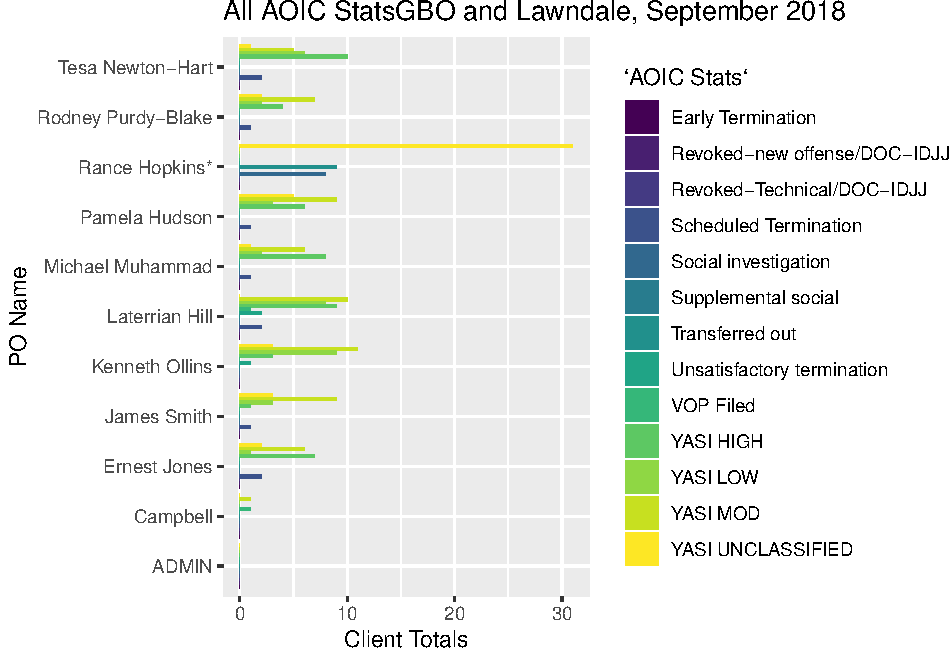
\includegraphics[width=0.9\linewidth,height=0.9\textheight,]{reporting_updates_files/figure-latex/initial_graphs-1} \caption{GBO and Lawndale, September 2018}\label{fig:initial_graphs}
\end{figure}

\newpage

And unlike Excel, this format easily lends itself to additional
visualizations, such as filtering results to focus on specific
variables, such as Social Investigations and VOP's Filed. For this
example, the background code is included to show how this work is done.

First as a chart:

\begin{Shaded}
\begin{Highlighting}[]
\NormalTok{cal_}\DecValTok{57} \OperatorTok
\StringTok{  }\KeywordTok{tidy_up}\NormalTok{() }\OperatorTok
\StringTok{  }\KeywordTok{bind_rows}\NormalTok{(lloyd) }\OperatorTok\StringTok{ }
\StringTok{  }\KeywordTok{select}\NormalTok{(}\DecValTok{1}\NormalTok{, }\StringTok{`}\DataTypeTok{Social Investigation}\StringTok{`}\NormalTok{ =}\StringTok{`}\DataTypeTok{Social investigation}\StringTok{`}\NormalTok{,}
         \StringTok{`}\DataTypeTok{VOP}\StringTok{`}\NormalTok{ =}\StringTok{ `}\DataTypeTok{VOP Filed}\StringTok{`}\NormalTok{) }\OperatorTok\StringTok{ }
\StringTok{  }\KeywordTok{filter}\NormalTok{(}\StringTok{`}\DataTypeTok{Social Investigation}\StringTok{`} \OperatorTok{>}\StringTok{ }\DecValTok{0} \OperatorTok{|}\StringTok{ }\NormalTok{VOP }\OperatorTok{>}\StringTok{ }\DecValTok{0}\NormalTok{) }\OperatorTok
\StringTok{  }\KeywordTok{kable}\NormalTok{(}\DataTypeTok{booktabs =} \OtherTok{TRUE}\NormalTok{, }\DataTypeTok{format =} \StringTok{"latex"}\NormalTok{, }
        \DataTypeTok{caption =} \StringTok{"GBO: September, 2018"}\NormalTok{) }\OperatorTok
\StringTok{  }\KeywordTok{kable_styling}\NormalTok{(}\DataTypeTok{latex_options =} \KeywordTok{c}\NormalTok{(}\StringTok{"striped"}\NormalTok{, }
                                  \StringTok{"hold_position"}\NormalTok{, }\StringTok{"scale_down"}\NormalTok{),}
                \DataTypeTok{stripe_color =} \StringTok{"lightgray"}\NormalTok{)}
\end{Highlighting}
\end{Shaded}

\rowcolors{2}{lightgray}{white}
\begin{table}[!h]

\caption{\label{tab:as_chart}GBO: September, 2018}
\centering
\resizebox{\linewidth}{!}{
\begin{tabular}[t]{lrr}
\hiderowcolors
\toprule
PO\_Name & Social Investigation & VOP\\
\midrule
\showrowcolors
Campbell & 0 & 1\\
Laterrian Hill & 0 & 1\\
Rance Hopkins* & 8 & 0\\
\bottomrule
\end{tabular}}
\end{table}
\rowcolors{2}{white}{white}

And as a graph:

\begin{Shaded}
\begin{Highlighting}[]
\NormalTok{lloyd <-}\StringTok{  }\NormalTok{cal_}\DecValTok{55}\NormalTok{_}\DecValTok{2} \OperatorTok\StringTok{ }
\StringTok{    }\KeywordTok{tidy_up}\NormalTok{() }

\NormalTok{cal_}\DecValTok{57} \OperatorTok
\StringTok{  }\KeywordTok{tidy_up}\NormalTok{() }\OperatorTok
\StringTok{  }\KeywordTok{bind_rows}\NormalTok{(lloyd) }\OperatorTok\StringTok{ }
\StringTok{  }\KeywordTok{select}\NormalTok{(}\DecValTok{1}\NormalTok{, }\StringTok{`}\DataTypeTok{Social Investigation}\StringTok{`}\NormalTok{ =}\StringTok{`}\DataTypeTok{Social investigation}\StringTok{`}\NormalTok{, }
         \StringTok{`}\DataTypeTok{VOP}\StringTok{`}\NormalTok{ =}\StringTok{ `}\DataTypeTok{VOP Filed}\StringTok{`}\NormalTok{) }\OperatorTok
\StringTok{  }\KeywordTok{gather}\NormalTok{( }\KeywordTok{c}\NormalTok{(}\StringTok{`}\DataTypeTok{Social Investigation}\StringTok{`}\NormalTok{, }\StringTok{`}\DataTypeTok{VOP}\StringTok{`}\NormalTok{), }\DataTypeTok{key =}\NormalTok{ Social_VOP, }
          \DataTypeTok{value =}\NormalTok{ Totals) }\OperatorTok
\StringTok{  }\KeywordTok{ggplot}\NormalTok{(}\KeywordTok{aes}\NormalTok{(}\DataTypeTok{x =}\NormalTok{ PO_Name, }\DataTypeTok{y =}\NormalTok{ Totals, }\DataTypeTok{fill =} \StringTok{`}\DataTypeTok{Social_VOP}\StringTok{`}\NormalTok{)) }\OperatorTok{+}\StringTok{ }
\StringTok{  }\KeywordTok{geom_bar}\NormalTok{(}\DataTypeTok{stat =} \StringTok{"identity"}\NormalTok{, }\DataTypeTok{position =} \StringTok{"dodge"}\NormalTok{) }\OperatorTok{+}
\StringTok{  }\NormalTok{viridis}\OperatorTok{::}\KeywordTok{scale_fill_viridis}\NormalTok{(}\DataTypeTok{discrete =} \OtherTok{TRUE}\NormalTok{, }\DataTypeTok{name =} \StringTok{"Socials and VOP"}\NormalTok{) }\OperatorTok{+}
\StringTok{  }\KeywordTok{labs}\NormalTok{(}\DataTypeTok{title =} \StringTok{"GBO and Lawndale, September 2018"}\NormalTok{,}
       \DataTypeTok{x =} \StringTok{"PO Name"}\NormalTok{, }\DataTypeTok{y =} \StringTok{"Client Totals"}\NormalTok{) }\OperatorTok{+}
\StringTok{  }\KeywordTok{coord_flip}\NormalTok{()}
\end{Highlighting}
\end{Shaded}

\begin{figure}
\centering
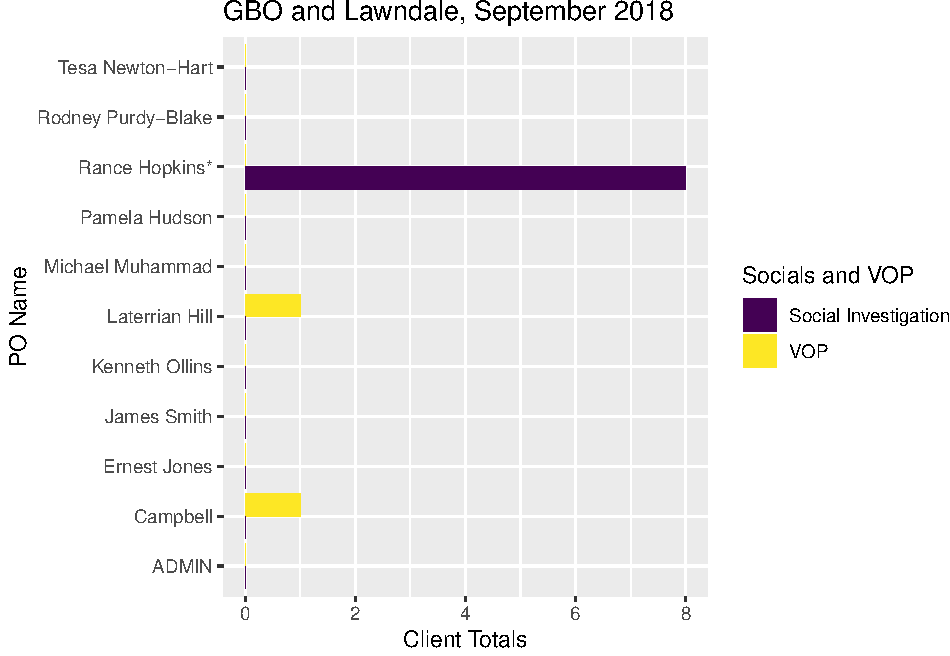
\includegraphics{reporting_updates_files/figure-latex/SI_VOP-1.pdf}
\caption{Socials and VOPs in GBO and Lawndale}
\end{figure}

In both of the previous examples, snippets of code were included in the
document to showcase how \texttt{R} handles filtering. What makes this
method superior to Excel is that the above code can be reused with a
similar dataset. For instance, plotting the same AOIC stas with Markham
North:

\begin{Shaded}
\begin{Highlighting}[]
\NormalTok{cal_mark_n }\OperatorTok
\StringTok{  }\KeywordTok{tidy_up}\NormalTok{() }\OperatorTok\StringTok{ }
\StringTok{  }\KeywordTok{select}\NormalTok{(}\DecValTok{1}\NormalTok{, }\StringTok{`}\DataTypeTok{Social Investigation}\StringTok{`}\NormalTok{ =}\StringTok{`}\DataTypeTok{Social investigation}\StringTok{`}\NormalTok{, }
         \StringTok{`}\DataTypeTok{VOP}\StringTok{`}\NormalTok{ =}\StringTok{ `}\DataTypeTok{VOP Filed}\StringTok{`}\NormalTok{) }\OperatorTok
\StringTok{  }\KeywordTok{gather}\NormalTok{( }\KeywordTok{c}\NormalTok{(}\StringTok{`}\DataTypeTok{Social Investigation}\StringTok{`}\NormalTok{, }\StringTok{`}\DataTypeTok{VOP}\StringTok{`}\NormalTok{), }\DataTypeTok{key =}\NormalTok{ Social_VOP, }
          \DataTypeTok{value =}\NormalTok{ Totals) }\OperatorTok
\StringTok{  }\KeywordTok{ggplot}\NormalTok{(}\KeywordTok{aes}\NormalTok{(}\DataTypeTok{x =}\NormalTok{ PO_Name, }\DataTypeTok{y =}\NormalTok{ Totals, }\DataTypeTok{fill =} \StringTok{`}\DataTypeTok{Social_VOP}\StringTok{`}\NormalTok{)) }\OperatorTok{+}\StringTok{ }
\StringTok{  }\KeywordTok{geom_bar}\NormalTok{(}\DataTypeTok{stat =} \StringTok{"identity"}\NormalTok{, }\DataTypeTok{position =} \StringTok{"dodge"}\NormalTok{) }\OperatorTok{+}
\StringTok{  }\NormalTok{viridis}\OperatorTok{::}\KeywordTok{scale_fill_viridis}\NormalTok{(}\DataTypeTok{discrete =} \OtherTok{TRUE}\NormalTok{, }\DataTypeTok{name =} \StringTok{"Socials and VOP"}\NormalTok{) }\OperatorTok{+}
\StringTok{  }\KeywordTok{labs}\NormalTok{(}\DataTypeTok{title =} \StringTok{"Markham North, September 2018"}\NormalTok{,}
       \DataTypeTok{x =} \StringTok{"PO Name"}\NormalTok{, }\DataTypeTok{y =} \StringTok{"Client Totals"}\NormalTok{) }\OperatorTok{+}
\StringTok{  }\KeywordTok{coord_flip}\NormalTok{()}
\end{Highlighting}
\end{Shaded}

\begin{figure}
\centering
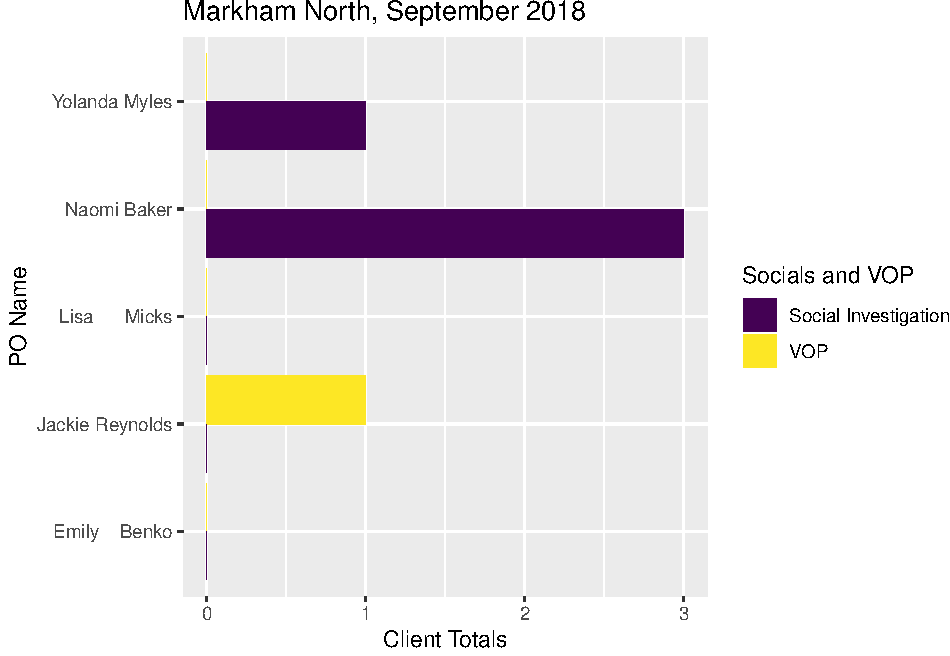
\includegraphics{reporting_updates_files/figure-latex/markham_north-1.pdf}
\caption{Socials and VOPs in Markham North}
\end{figure}

With Excel, each months need to be recalculated from the specific sheet.
With \texttt{R}, the code can be reused with limited changes.

With additional resources, specifically installing free software on a
the Chief Judge's server, the department would be able to run these same
reports internally as a website. This software, known as
\href{https://shiny.rstudio.com}{Shiny}, would allow us to create
dashboards and programmable reports that can updated quickly. Additional
examples of how Shiny can be used can be found
\href{https://shiny.rstudio.com/gallery/}{here.}

\hypertarget{resources}{%
\section{Resources}\label{resources}}

\texttt{CFive\ Supervisor} will encourage the department to continue
down a data driven path. Maximizing the return on this investment
requires additional departmental resources, the minimum of which is a
system administrator to ensure data integrity. Just doing the minimum,
however, will not make the most of this new system (and the changes to
procedure that is sure to follow.) To this end, a new unit should be
created to ensure that handles all department data and visualizations.
This would include the short term goals of changing the AOIC stat format
to a Tidy one and as well as producing stats until
\texttt{CFive\ Supervisor\textquotesingle{}s} is fully implemented, as
well as long term goals of using our data to ensure the creation of data
driven policies, procedures, and programs:

\emph{It is the policy of the Cook County Juvenile Probation and Court
Services Department to maintain the highest level of data integrity
within the department and with community partners and to use this data
to develop polices, procedures, and programs that enhance the
possibility of long term success for all young people under the care of
the court.}

This unit would house:

\begin{itemize}
\tightlist
\item
  Two support professionals to help collect data and generate reports
  and visualizations.
\item
  The CFive System Administrator
\end{itemize}

Two such individuals already do this work in the department, so
including them in this new department would only service to solidify
this commitment to data driven approaches. The role of CFive Systems
Administrator will need to be a permanent position for maintaining the
systemt; therefore it is logical to add this position to a unit that is
focused on data.

In addition to reporting and collection tasks, the supervisor of the
unit would also be responsible for maintain and leverage all of the data
sharing agreements the department has with other justice and community
agencies. Other staff maybe needed to help develop programs that stem
from the insights gained by maximizing the utility of
\texttt{CFive\ Supervisor}; shifting staff resources to this new unit
would suffice for current needs. In creating this unit, the department
frames data as a ``mission critical'' aspect, and redistributes all of
the varied data tasks under one roof. It is not a revolutionary change,
simple an evolution of the departments needs, capabilities, and
opportunities.


\end{document}
